\begin{theo}[Verplaatsingsstroom]{Verplaatsingsstroom}
    De verplaatsingsstroom is een `stroom' die ontstaat door een veranderend elektrisch veld, bv in een condensator. De verplaatsingsstroom is gegeven door
    \begin{equation*}
        I_d = \epsilon_0 \frac{d\Phi_E}{dt} = \epsilon_0 \frac{d}{dt} \oint \Vec{E} \cdot d\Vec{A}
    \end{equation*}
    waarbij $ \Phi_E $ de elektrische flux is.
    De totale verplaatsingsstroom is gelijk aan de geleidingsstroom, bv de stroom geleverd aan de condensator.

    \vspace{0.3cm}
    \noindent \textbf{Opmerking:} de naam is een verwijzing naar een oude, verworpen theorie; noch is de verplaatsingsstroom een echte stroom van ladingen, noch is er een verplaatsing
\end{theo}

\begin{lem}[Ampère-Maxwell]{Ampère-Maxwell}
    De wet Ampère-Maxwell beweert dat bewegende elektrische ladingen en veranderende elektrische velden magnetische velden opwekken, in formulevorm:
    \begin{equation*}
        \oint \Vec{B} \cdot d\Vec{\ell}
        = \mu_0 ( I_C + I_d ) 
        % &= \mu_0 \left( I + \epsilon_0 \frac{d\Phi_E}{dt} \right) 
        = \mu_0 I_C + \mu_0 \epsilon_0 \frac{d\Phi_E}{dt} 
        % = \mu_0 I + \mu_0 \epsilon_0 \frac{d}{dt} \oint \Vec{E} \cdot d\Vec{A}
    \end{equation*}
    waarbij $ I_C $ de \textbf{geleidingsstroom} en $ I_d $ de \textbf{verplaatsingsstroom} is. Deze stelt de stroom voor die ontstaat door een veranderend elektrisch veld. 
\end{lem}

\begin{lem}[Gauss voor Magnetisme]{Gauss voor Magnetisme}
    Het is algemeen aanvaard dat magnetische monopoles niet bestaan. Dit betekent dat de magnetische flux door een gesloten oppervlak altijd nul is, in formulevorm
    \begin{equation*}
        \oint \Vec{B} \cdot d\Vec{A} = 0
    \end{equation*}
    \vspace{-0.5cm}
\end{lem}

% \begin{vrg}[Gauss]{Gauss}
%     \vspace{-0.3cm}
%     \def\arraystretch{2}
%     \hspace{1.5cm}
%     \begin{tabular}{c|c}
%         Elektrische velden & Magnetische velden \\ \hline
%         $\oint \Vec{E} \cdot d\Vec{A} = \frac{q_{\text{in}}}{\epsilon_0}$ &  $\oint \Vec{B} \cdot d\Vec{A} = 0$ \\
%         Bron: elektrische ladingen & Bron: bewegende elektrische ladingen \\
%         elektrische veldlijnen kunnen open zijn & magnetische veldlijnen zijn gesloten \\
%     \end{tabular}
% \end{vrg}

% \newpage

\begin{summ}[Vergelijkingen van Maxwell]{Vergelijkingen van Maxwell}
    \vspace{-0.3cm}
    \begin{center}
        \def\arraystretch{2}
        \begin{tabular}{c|c}
            Elektrisch veld & Magnetisch veld \\ \hline
            $\oint \Vec{E} \cdot d\Vec{A} = \frac{Q}{\epsilon_0}$ 
                &  $\oint \Vec{B} \cdot d\Vec{A} = 0$ \\
            $\oint \Vec{E} \cdot d\Vec{\ell} = -\frac{d\Phi_B}{dt}$ 
                &  $\oint \Vec{B} \cdot d\Vec{\ell} = \mu_0I + \mu_0 \epsilon_0 \frac{d\Phi_B}{dt}$ \\
        \end{tabular}
    \end{center}
\end{summ}

\newpage

\begin{theo}[Golfvergelijking]{Golfvergelijking}
    Een golf kunnen we wiskundig voorstellen als een functie van de vorm
    \begin{equation*}
        D(x,t) = A\sin(kx-\omega t) \quad \text{met} \quad \frac{\partial^2 D}{\partial x^2} = \frac{1}{v^2} \frac{\partial^2 D}{\partial t^2}
    \end{equation*}
    \vspace{-0.3cm}
\end{theo}

\begin{app}[Vlakke golven]{Vlakke golven}
    \vspace{-0.2cm}
    \begin{minipage}{.7\textwidth}
        We kunnen de derde wet van Maxwell toepassen om de snelheid van hetzij een elektrische vlakke golf, hetzij een magnetische vlakke golf te bepalen. Herneem de derde wet van Maxwell:
        \begin{equation}
            \oint \Vec{E} \cdot d\Vec{\ell} = -\frac{d\Phi_B}{dt}.
        \end{equation}
        Indien we het pad nemen zoals in de figuur, dan is de potentiaal door het pad gelijk aan:
    \end{minipage}
    \begin{minipage}{.26\textwidth  }
        \vspace{-0.1cm}\hspace{0.3cm}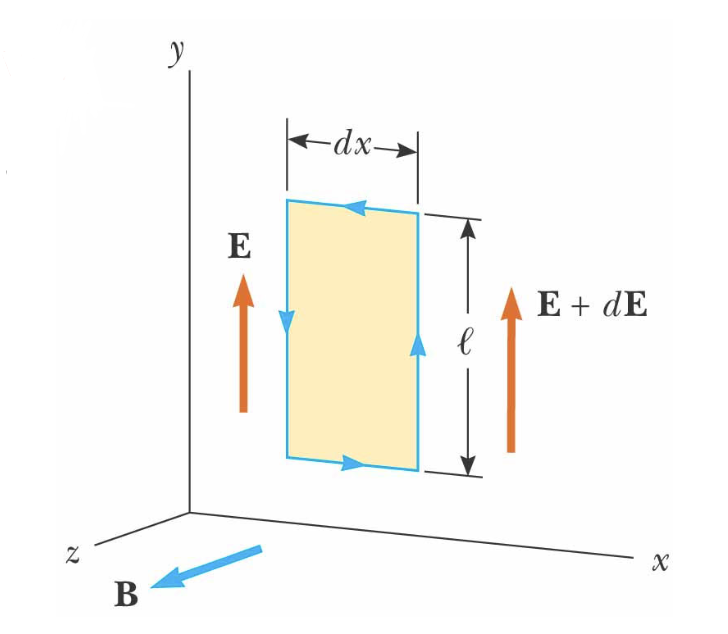
\includegraphics[scale = 0.17]{Images/Magnetisme/GeslotenPadVlakkeGolf.png}
    \end{minipage}
    \begin{equation}
        \oint \Vec{E} \cdot d\Vec{\ell} = \left[E(x+ dx, t)\right]\ell - \left[E(x,t)\right]\ell \approx \ell\left(\frac{\partial E}{\partial x}\right)dx.
    \end{equation}
    De magnetische flux vinden we als volgt:
    \begin{equation}
        \frac{d\Phi_B}{dt} = \frac{d}{dt}\left[B(x,t)\ell dx\right] = \ell dx\frac{\partial B}{\partial t}.    
    \end{equation}
    Als we nu (2) en (3) invullen in (1), dan vinden we
    \begin{equation*}
        \frac{\partial E}{\partial x} = - \frac{\partial B}{\partial t}
    \end{equation*}
    of analoog als we de magnetische vlakke golf beschouwen (dan met de vierde wet van Maxwell)
    \begin{equation*}
        \frac{\partial B}{\partial x} = - \mu_0\epsilon_0 \frac{\partial E}{\partial t}.
    \end{equation*}
    Hieruit kunnen we de volgende twee golfformules afleiden
    \begin{center}
        \def\arraystretch{2}
        \begin{tabular}{c|c}
            Vlakke elektrisch golf & Vlakke magnetisch golf \\ \hline
            $\frac{\partial^2 E}{\partial x^2} = \mu_0\epsilon_0 \frac{\partial^2 E}{\partial t^2} $ & $\frac{\partial^2 B}{\partial x^2} = \mu_0\epsilon_0 \frac{\partial^2 B}{\partial t^2}$ 
        \end{tabular}
    \end{center}
    waaruit we dus de snelheid van de golven kunnen afleiden
    \begin{equation*}
        v = \frac{1}{\sqrt{\mu_0\epsilon_0}} = c.
    \end{equation*}
    % uit de algemene golfformule
    % \begin{equation*}
    %     \frac{\partial^2 D}{\partial x^2} = \frac{1}{v^2} \frac{\partial^2 D}{\partial t^2} \quad \text{waarbij} \quad D(x,t) = A\sin(kx-\omega t).
    % \end{equation*}
    \vspace{0.3cm}
    \textbf{Opmerking:} licht is dus ook een elektromagnetische golf!
\end{app}

\newpage

\begin{pro}[Eigenschappen van elektromagnetische straling]{Eigenschap van elektromagnetische straling}
    \begin{itemize}
        \item
            De oplossing van de derde en vierde Maxwell vergelijking is een elektromagnetische golf (zie vorige pagina).
        \item 
            Bij een elektromagnetische golf is op elk ogenblik de verhouding tussen de grootte van het elektrisch veld en de grootte van het magnetisch veld gelijk aan de lichtsnelheid $ c $, ofwel:
            \begin{equation*}
                \frac{E_{\text{max}}}{B_{\text{max}}} = \frac{E}{B} = c.
            \end{equation*}
        \item 
            Bij een vlakke golf staan $E$ en $B$ loodrecht op elkaar, en loodrecht op de voortplantingsrichting: \textbf{transversale golf}.
    \end{itemize}
    \begin{center}
        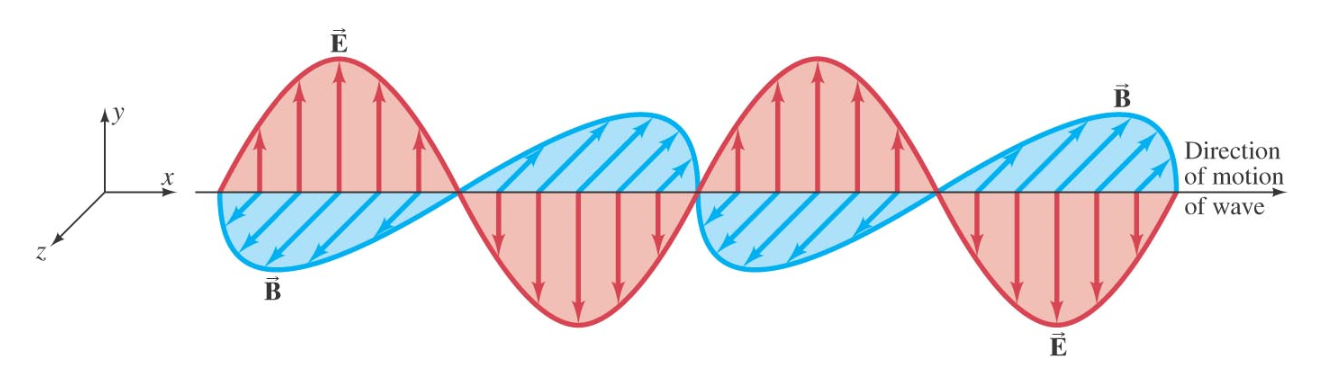
\includegraphics[scale = 0.175]{Images/Magnetisme/ElektromagnetischeStraling.png}
    \end{center}
    \vspace{-0.3cm}
\end{pro}

\begin{theo}[Energie in elektromagnetische golven]{Energie in elektromagnetische golven}
    Elektromagnetische golven brengen energie over. De energiedichtheid van een elektromagnetische golf is gegeven door
    \begin{equation*}
        u = \frac{1}{2}\epsilon_0 E^2 + \frac{1}{2}\frac{B^2}{\mu_0}
    \end{equation*}
    wat we kunnen vereenvoudigen, sinds $\frac{E}{B}=c$:
    \begin{equation*}
        u = \epsilon_0 E^2 = \frac{B^2}{\mu_0} = \sqrt{\frac{\epsilon_0}{\mu_0}}EB.
    \end{equation*}
    \vspace{-0.3cm}
\end{theo}

\begin{theo}[Poyntingvector]{Poyntingvector}
    De Poyntingvector is een vector van een elektromagnetische golf 
    \begin{equation*}
        \Vec{S} = \frac{1}{\mu_0}\left(\Vec{E} \times \Vec{B}\right)
    \end{equation*}
    met
    \begin{itemize}
        \item richting: de voortplantingsrichting van de golf
        \item grootte: de energie per tijd én per oppervlakte
    \end{itemize}
\end{theo}